\let\negmedspace\undefined
\let\negthickspace\undefined
\documentclass[journal]{IEEEtran}
\usepackage[a5paper, margin=10mm, onecolumn]{geometry}
%\usepackage{lmodern} % Ensure lmodern is loaded for pdflatex
\usepackage{tfrupee} % Include tfrupee package

\setlength{\headheight}{1cm} % Set the height of the header box
\setlength{\headsep}{0mm}     % Set the distance between the header box and the top of the text

\usepackage{gvv-book}
\usepackage{gvv}
\usepackage{cite}
\usepackage{amsmath,amssymb,amsfonts,amsthm}
\usepackage{algorithmic}
\usepackage{graphicx}
\usepackage{textcomp}
\usepackage{xcolor}
\usepackage{txfonts}
\usepackage{listings}
\usepackage{enumitem}
\usepackage{mathtools}
\usepackage{gensymb}
\usepackage{comment}
\usepackage[breaklinks=true]{hyperref}
\usepackage{tkz-euclide} 
\usepackage{listings}

% \usepackage{gvv}                                        
\def\inputGnumericTable{}                                 
\usepackage[latin1]{inputenc}                                
\usepackage{color}                                            
\usepackage{array}                                            
\usepackage{longtable}                                       
\usepackage{calc}                                             
\usepackage{multirow}                                         
\usepackage{hhline}                                           
\usepackage{ifthen}                                           
\usepackage{lscape}
\begin{document}

\bibliographystyle{IEEEtran}
\vspace{3cm}


\renewcommand{\thefigure}{\theenumi}
\renewcommand{\thetable}{\theenumi}
\setlength{\intextsep}{10pt} % Space between text and floats


\numberwithin{equation}{enumi}
\numberwithin{figure}{enumi}
\renewcommand{\thetable}{\theenumi}

\title{GATE ME-2007}
\author{AI24BTECH11001 - Abhijeet Kumar
}
\maketitle
\renewcommand{\thefigure}{\theenumi}
\renewcommand{\thetable}{\theenumi}

\begin{enumerate}[start = 52]
    \item The natural frequemcy of the system shown below is
    \begin{figure}[h]
    \centering
    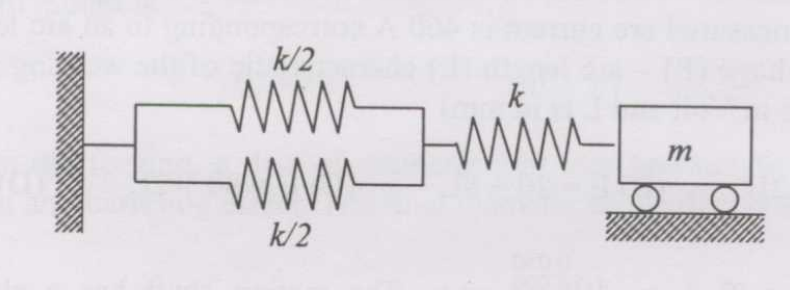
\includegraphics[width=0.5\textwidth]{fig1.png}  
    \end{figure}

    \begin{multicols}{4}
        \begin{enumerate}
            \item $\sqrt{\frac{k}{2m}}$
            \item $\sqrt{\frac{k}{m}}$
            \item $\sqrt{\frac{2k}{m}}$
            \item $\sqrt{\frac{3k}{m}}$
        \end{enumerate}
    \end{multicols}

    \item The equation of motion for a harmonic oscillator is given by:
    \begin{align*}
    {\frac{d^2 x}{dt^2}} + 2\zeta \omega_n \frac{dx}{dt} + \omega_n^2 x = 0
    \end{align*}
    and the initial condition at $t = 0$ are $x\brak{0}$ = $X$ ,$ \frac{dx}{dt}\brak{0} = 0$. The amplitude of $x\brak{t}$ after n complete cycles is
    \begin{multicols}{2}
    \begin{enumerate}
        \item $X e^{-2n\pi \brak{\frac{\zeta}{\sqrt{1 - \zeta^2}}}}$
        \item $X e^{2n\pi \brak{\frac{\zeta}{\sqrt{1 - \zeta^2}}}}$
        \item $X e^{-2n\pi \brak{\frac{\sqrt{1 - \zeta^2}}{\zeta}}}$
        \item $X$
    \end{enumerate}
    \end{multicols}

    \item The piston rod of diameter $20$ mm and length $ 700$ mm in a hydraulic cylinder is subjected to a compressive force of $10$ kN due to the internal pressure. The end conditions for the rod may be assumed as guided at the piston end and hinged at the other end. The Young's modulus is $200$ GPa. The factor of safety for the piston rod is
     \begin{multicols}{4}
        \begin{enumerate}
            \item $0.68$
            \item $2.75$
            \item $5.62$
            \item $11.0$
        \end{enumerate}
    \end{multicols}

    \item In electrodischarge machining (EDM), if the thermal conductivity of tool is high and the specific heat of work piece is low, then the tool wear rate and material removal rate are expected to be respectively
     \begin{multicols}{2}
    \begin{enumerate}
        \item high and high
        \item low and low
        \item high and low
        \item low and high
    \end{enumerate}
    \end{multicols}

    \item In orthogonal turning of medium carbon steel, the specific machining energy is $2.0$ J/$mm^{3}$. The cutting velocity, feed and depth of cut are $120$ m/min, $0.2$ mm/rev and $2$ mm respectively. The main cutting force in N is
    \begin{multicols}{4}
        \begin{enumerate}
            \item $40$
            \item $80$
            \item $400$
            \item $800$
        \end{enumerate}
    \end{multicols}

    \item A direct current welding machine with a linear power source characteristic provides open circuit voltage of $80$ V and short circuit current of $800$ A. During welding with the machine, the measured arc current is $500$ A corresponding to an arc length of $5.0$ mm and the measured arc current is $460$ A corresponding to an arc length of $7.0$ mm. The linear voltage (E) arc length (L) characteristic of the welding arc can be given as (where E is in Volt and L is in mm)
    \begin{multicols}{4}
        \begin{enumerate}
            \item E = 20 + 2L
            \item E = 20 + 8L
            \item E = 80 + 2L
            \item E = 80 + 8L
        \end{enumerate}
    \end{multicols}

    \item A hole is specified as $40^{\begin{matrix} 0.050 \\ 0.000 \end{matrix}}$ mm. The mating shaft has a clearance fit with minimum clearance of $0.01$ mm. The tolerance on the shaft is $0.04$ mm. The maximum clearance in mm between the hole and the shaft is
    \begin{multicols}{4}
        \begin{enumerate}
            \item $0.04$
            \item $0.05$
            \item $0.10$
            \item $0.11$
        \end{enumerate}
    \end{multicols}

    \item In orthogonal turning of low carbon steel pipe with principal cutting edge angle of $90^{0}$ the main cutting force is $1000$ N and the feed force is $800$ N. The shear angle is $25^{0}$ and orthogonal rake angle is zero. Employing Merchant's theory, the ratio of friciton force to normal force acting on the cutting tool is
    \begin{multicols}{4}
        \begin{enumerate}
            \item $1.56$
            \item $1.25$
            \item $0.80$
            \item $0.64$
        \end{enumerate}
    \end{multicols}

    \item Two metallic sheets, each of $2.0$ mm thickness, are welded in a lap joint configuration by resistance spot welding at a welding current of $10$ kA and welding time of $10$ millisecond. A spherical fusion zone extending up to the full thickness of each sheet is formed. The properties of the metallic sheets are given as:

    ambient temperature = $293$ K \\
    melting temperature = $1793$ K \\
    latent heat of fusion = $300$ kJ/kg\\
    density = $7000$ kg/$m^{3}$ \\
    specific heat $800$ J/kgK\\
    Assume: $\brak{i}$ contact resistance along sheet-sheet interface is $500$ micro-ohm and along electrode-sheet interface' is zero; $\brak{ii}$ no conductive heat loss through the bulk sheet materials; and $\brak{iii}$ the complete weld fusion zone is at the melting temperature.\\

    The melting efficiency $\brak{in \%}$ of the process is
    \begin{multicols}{4}
        \begin{enumerate}
            \item $50.37$
            \item $60.37$
            \item $70.37$
            \item $80.37$
        \end{enumerate}
    \end{multicols}

    \item Capacities of production of an item over $3$ consecutive months in regular time are $100$, $100$ and $80$ and in overtime are $20$, $20$ and $40$. The demands over those $3$ months are $90$, $130$ and $110$. The cost of production in regular time and overtime are respectively Rs. $20$ per item and Rs. $24$ per item. Inventory carrying cost is Rs. $2$ per item per month, The levels of starting and final inventory are nil. Backorder is not permitted. For minimum cost of plan, the level of planned production in overtime in the third month is
    \begin{multicols}{4}
        \begin{enumerate}
            \item $40$
            \item $30$
            \item $20$
            \item $0$
        \end{enumerate}
    \end{multicols}

    \item In open-die forging, a disc of diameter $200$ mm and height $60$ mm is compressed without any barreling effect. The final diameter of the disc is is 400 mm. The true strain is 
    \begin{multicols}{4}
        \begin{enumerate}
            \item $1.986$
            \item $1.686$
            \item $1.386$
            \item $0.602$
        \end{enumerate}
    \end{multicols}

    \item The thickness of a metallic sheet is reduced from an initial value of $16$ mm to a final value of $10$ mm in one single pass rolling with a pair of cylindrical rollers each of diameter of $400$ mm. The bite angle in degree will be
    \begin{multicols}{4}
        \begin{enumerate}
            \item $5.936$
            \item $7.936$
            \item $8.936$
            \item $9.936$
        \end{enumerate}
    \end{multicols}

    \item Match the correct combination for following metal working processes
    \begin{multicols}{2}
			\textbf{Processes}
			\begin{enumerate}[label=(\Alph*)]
                
				\item Blanking
				\item Stretch Forming
                    \item Coining
                    \item Deep Drawing
			\end{enumerate}
			\columnbreak
			\textbf{Associated state of stress}
			\begin{enumerate}[label=(\arabic*)]
				\item Tension
				\item Compression
				\item Shear
                    \item Tension and Compression
                    \item Tension and Shear
			\end{enumerate}
		\end{multicols}

      \begin{multicols}{2}
        \begin{enumerate}
            \item $A-2,B-1,C-3,D-4$
            \item $A-3,B-4,C-1,D-5$
            \item $A-5,B-4,C-3,D-1$
            \item $A-3,B-1,C-2,D-4$
        \end{enumerate}
    \end{multicols}

    \item A $200$ mm long down sprue has an area of cross-section of $650$ $mm^2$ where the pouring basin meets the down sprue (i.e. at the beginning of the down sprue). A constant head of molten metal is maintained by the pouring basin. The molten metal flow rate is $6.5 \times 10^5$ $mm^{3}/s$. Considering the end of down sprue to be open to atmosphere and an acceleration due to gravity of $10^4$ $mm/s^2$, the area of the down sprue in $mm^2$ at its end (avoiding aspirat effect) should be
    \begin{figure}[h]
    \centering
    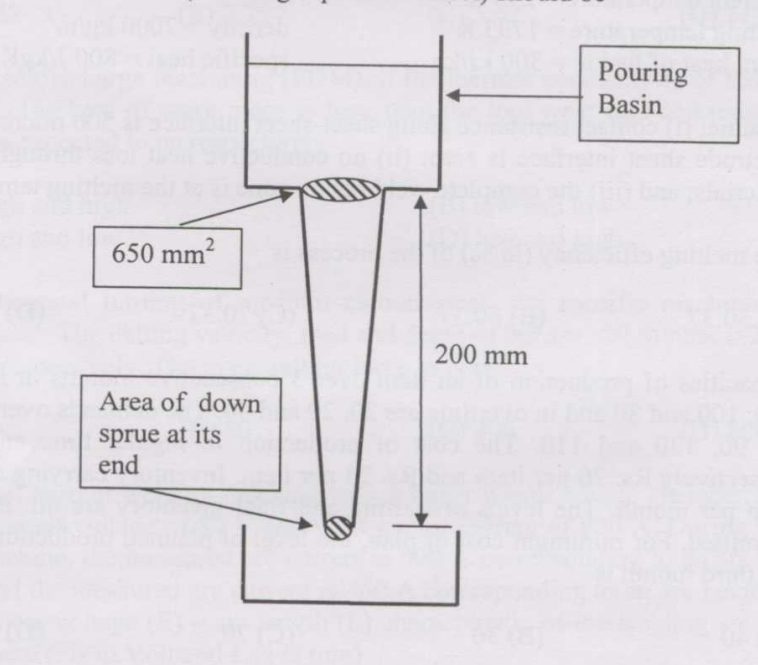
\includegraphics[width=0.5\textwidth]{fig2.png} 
    \end{figure}

     \begin{multicols}{4}
        \begin{enumerate}
            \item $650.0$
            \item $350.0$
            \item $290.7$
            \item $190.0$
        \end{enumerate}
    \end{multicols}

    \item The force requirement in a blanking operation of low carbon steel sheet is $5.0$ kN. The thickness of the sheet is 't' and diameter of the blanked part is 'd'. For the same work material, if the diameter of the blanked part is increased to $1.5$ d and thickness is reduced to $0.4$ t, the new blanking force in kN is
    \begin{multicols}{4}
        \begin{enumerate}
            \item $3.0$
            \item $4.5$
            \item $5.0$
            \item $8.0$
        \end{enumerate}
    \end{multicols}

    \item Match the most suitable manufacturing processes for the following parts
        \begin{multicols}{2}
			\textbf{Parts}
			\begin{enumerate}[label=(\Alph*)]
                
				\item Computer chip
				\item Metal forming dies and molds
                    \item Turbine blade
                    \item Glass
			\end{enumerate}
			\columnbreak
			\textbf{Manufacturing Processes}
			\begin{enumerate}[label=(\arabic*)]
				\item Electrochemical Machining
				\item Ultrasonic Machining
				\item Electrodischarge Machining
                    \item Photochemical Machining
			\end{enumerate}
		\end{multicols}

      \begin{multicols}{2}
        \begin{enumerate}
            \item $A-4,B-3,C-1,D-2$
            \item $A-4,B-3,C-2,D-1$
            \item $A-3,B-1,C-4,D-2$
            \item $A-1,B-2,C-4,D-3$
        \end{enumerate}
    \end{multicols}

    \item The maximum level of inventory of an item is $100$ and it is achieved with infinite replenishment rate. The inventory becomes zero over one and half month due to consumption at a uniform rate. This cycle continues throughout the year. Ordering cost is Rs. $100$ per order and inventory carrying cost is Rs. 10 per item per month. Annual cost$ \brak{IN rS.}$ of the plan, neglecting material cost, is
    \begin{multicols}{4}
        \begin{enumerate}
            \item $800$
            \item $2800$
            \item $4800$
            \item $6800$
        \end{enumerate}
    \end{multicols}
    
\end{enumerate}

\end{document}
